\documentclass{llncs}
\usepackage[american]{babel}
\usepackage[T1]{fontenc}
\usepackage{times}
\usepackage{graphicx}
\usepackage[utf8]{inputenc}
\usepackage{booktabs}
%%%%%%%%%%%%%%%%%%%%%%%%%%%%%%%%%%%%%%%%%%%%%%%%%%%%%%%%%%%%%%%%%%%%%%%%
\begin{document}

\title{Author Profiling using SVMs\\and Word Embedding Averages}
%%% Please do not remove the subtitle.
\subtitle{Notebook for PAN at CLEF 2016}

\author{Roy Bayot \and Teresa Gonçalves}
\institute{Departamento de Informática, Escola de Ciências e
Tecnologia, \\Universidade de Évora, Rua Romão Ramalho,
59, 7000-671 Évora, Portugal \\  \email{d11668@alunos.uevora.pt, tcg@uevora.pt}}

\maketitle

\begin{abstract}
Briefly describe the main ideas of your approach.
\end{abstract}


\section{Introduction}
The specific problem associated with PAN 2016's task of author profiling involves the use of training data from a specific corpus and evaluated on a different corpus. The profiling was done in two different dimensions - age and gender classification. The training sets are also available in three different languages - English, Spanish, and Dutch. 

In previous author profiling research, most of the work is centered on hand crafted features as well as that which are content-based and style-based. For instance, in the work of Argamon et al. in~\cite{argamon2009automatically} where texts were categorized based on gender, age, native language, and personality, different content-based features and style-based features were used. In another example of Schler et al. in~\cite{schler2006effects} where writing styles in blogs are related to age and gender. Stylistic and content features were extracted from 71,000 different blogs and a Multi-Class Real Winnow was used to learn the models to classify the blogs. Stylistic features included parts-of-speech tags, function words, hyperlinks, and non-dictionary words. Content features included word unigrams with high information gain. %The accuracy achieved was around 80\% for gender classification and 75\% for age identification.

This can also be seen in the previous PAN editions. In the first edition of PAN~\cite{rangel2013overview} in 2013, the task  was age and gender profiling for English and Spanish blogs. There were a variety of methods used. One set includes content-based features such as bag of words, named entities, dictionary words, slang words, contractions, sentiment words, and emotion words. Another would be stylistic features such as frequencies, punctuations, POS, HTML use, readability measures, and other various statistics. There are also features that are n-grams based, IR-based, and collocations-based. Named entities, sentiment words, emotion words, and slang, contractions and words with character flooding were also considered. The work of Lopez-Monroy in~\cite{lopez2013inaoe} was considered the winner for the task although they placed second for both English and Spanish where they used second order representation based on relationships between documents and profiles. The work of Meina et al.~\cite{meina2013ensemble} used collocations and placed first for English while the work of Santosh et al. in~\cite{santosh2013author} worked well with Spanish using POS features.

In PAN 2014~\cite{rangel2014overview}, the task was profiling authors with text from four different sources - social media, twitter, blogs, and hotel reviews. Most of the approaches used in this edition are similar to the previous year. In~\cite{lopezusing}, the method used to represent terms in a space of profiles and then represent the documents in the space of profiles and subprofiles were built using expectation maximization clustering. This is the same method as in 2013 in~\cite{lopez2013inaoe}. In~\cite{maharjansimple}, n-grams were used with stopwords, punctuations, and emoticons retained, and then idf count was also used before placed into a classifier. Liblinear logistic regression returned with the best result. In~\cite{weren6exploring}, different features were used that were related to length (number of characters, words, sentences), information retrieval (cosine similarity, okapi BM25), and readability (Flesch-Kincaid readability, correctness, style). Another approach is to use term vector model representation as in~\cite{villenadaedalus}. For the work of Marquardt et al. in~\cite{marquardt2014age}, they used a combination of content-based features (MRC, LIWC, sentiments) and stylistic features (readability, html tags, spelling and grammatical error, emoticons, total number of posts, number of capitalized letters number of capitalized words). Classifiers also varied for this edition. There was the use of logistic regression, multinomial Naïve Bayes, liblinear, random forests, Support Vector Machines, and decision tables. The method of Lopez-Monroy in~\cite{lopezusing} gave the best result with an average accuracy of 28.95\% on all corpus-types and languages.

In PAN 2015~\cite{rangel2015overview}, the task was limited to tweets but expanded to different languages with age and gender classification and a personality dimension. The different languages include English, Spanish, Italian, and Dutch. There were 5 different personality dimensions - extroversion, stability, agreeableness, conscientiousness, and openness. And in this edition, the work of Alvarez-Carmona et al.~\cite{alvarezinaoe} gave the best results on English, Spanish, and Dutch. Their work used second order profiles as in the previous years as well as LSA. On the other hand, the work of Gonzales-Gallardo et al.~\cite{gonzaleztweets} gave the better result for Italian. This used stylistic features represented by character n-grams and POS n-grams.

Since the current task is to train on one type of corpus and test on another type of corpus, we decided to try an approach that uses word embeddings. We used word2vec in particular as described in~\cite{mikolov2013efficient}~\cite{mikolov2013distributed}. Such embeddings were trained not on the corpus given by PAN but by Wikipedia dumps so there is a possibility that using such embeddings which work on one corpus type could work on another corpus type. Our approach also uses these embeddings in conjunction with Support Vector Machines.


\section{Methodology}
The methodology is illustrated by the figure~\ref{System}. It mainly consists of three parts - word embedding creation, training, and evaluation. These will be further discussed in the subsequent subsections.

\begin{figure}
\centering
\caption{Overview of the system}
\label{System}
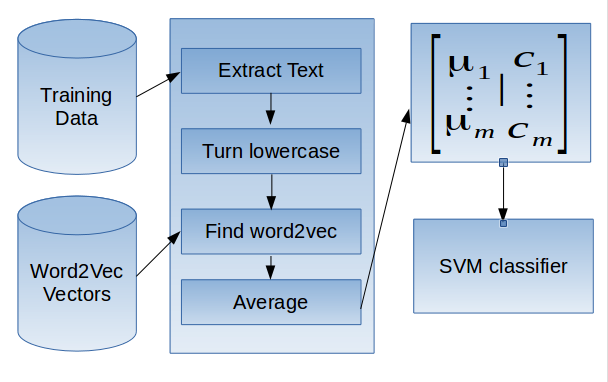
\includegraphics[scale=.5]{System.png}
\end{figure}


\subsection{Word Embeddings Creation}
Word embeddings were created. This was illustrated in the figure~\ref{W2vFlow} where wikipedia dumps are used as an input to the word2vec implementation of gensim~\cite{rehurek_lrec}. The wikipedia dump used for the following experiments were that of 05-02-2016. As for word2vec parameters, no lemmatization was done, the window size used was 5, and the output dimensions used was 100. The default continuous bag of words was also used. For further details, please refer to the tutorial given in~\cite{TrainWord2Vec}.

\begin{figure}
\centering
\caption{Overview of word2vec flow.}
\label{W2vFlow}
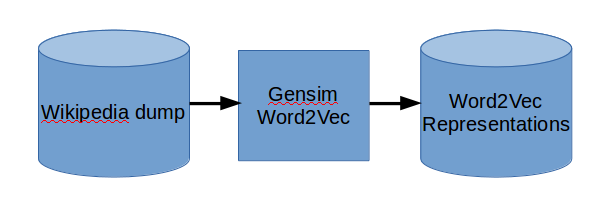
\includegraphics[scale=.5]{Word2Vec.png}
\end{figure}
\subsection{Training and Evaluation}
After obtaining word2vec representations for each word, each xml document of one twitter user is converted into word2vec representations. To do this, the texts were first extracted from the file. Then it was converted to lower case. After the conversion, the words are checked against the dictionary of all the words that have word2vec representations. If the words exists in the dictionary, the vector representation is pulled out and accumulated, and later normalized by the number of words that could be found in the dictionary. If the word does not exist in the dictionary, a zero vector is returned. 

After representing each twitter user, the vectors are then used as features. Support Vector Machines were then trained using those features. Different kernels and parameters were also checked. This includes polynomial kernel and a radial basis function. For the polynomial kernel, the degrees were restricted to 1, 2, and 3. The C parameter was restricted to 0.01, 1, 100. For the radial basis function, the gammas and C parameters were restricted to 0.01, 1, 100.

The performance of the system was evaluated using the accuracy measure and 10 fold cross validation was used. The parameters that gave the highest accuracies were noted and used in the system deployed in the TIRA server. 

\section{Results and Discussion}
The tables~\ref{EnglishAge}-~\ref{DutchAge} give the all the results for English, Spanish, and Dutch on age and gender. Looking at table~\ref{EnglishAge} for age classification in English, the highest accuracy obtained is 44.8\%. The SVM parameter that gave the best classification is the one with the radial basis function kernel with C to be 1 and gamma to be 100 although most of the other values are close. In gender classification however, the highest accuracy obtained was 68.2\% using a polynomial kernel with the degree to be 3 and C to be 100. There is more variety from these results given that the lowest is around 50.0\%.
\begin{table}[!htbp]
\centering
\caption{Age Classification Results for English}
\label{EnglishAge}
\begin{tabular}{cccccccc}
\toprule
     & \multicolumn{3}{c}{poly}   &  & \multicolumn{3}{c}{rbf}        \\
     & \multicolumn{3}{c}{degree} &  & \multicolumn{3}{c}{gamma}      \\
C    & 1       & 2       & 3      &  & 0.01  & 1     & 100            \\
\midrule
0.01 & 0.418   & 0.416   & 0.416  &  & 0.414 & 0.414 & 0.414          \\
1    & 0.418   & 0.416   & 0.416  &  & 0.414 & 0.418 & \textbf{0.448} \\
100  & 0.418   & 0.423   & 0.393  &  & 0.416 & 0.409 & 0.426         \\
\bottomrule 
\end{tabular}
\end{table}

\begin{table}[!htbp]
\centering
\caption{Gender Classification Results for English}
\label{EnglishGender}
\begin{tabular}{cccccccc}
\toprule
     & \multicolumn{3}{c}{poly}       &  & \multicolumn{3}{c}{rbf}   \\
     & \multicolumn{3}{c}{degree}     &  & \multicolumn{3}{c}{gamma} \\
C    & 1     & 2     & 3              &  & 0.01    & 1       & 100   \\
\midrule
0.01 & 0.534 & 0.495 & 0.495          &  & 0.498   & 0.500   & 0.512 \\
1    & 0.534 & 0.561 & 0.579          &  & 0.498   & 0.563   & 0.643 \\
100  & 0.534 & 0.677 & \textbf{0.682} &  & 0.548   & 0.672   & 0.643 \\
\bottomrule
\end{tabular}
\end{table}

The results for Spanish tweets are given below. In table~\ref{SpanishAge}, the highest accuracy for age classification is 51.3\%. This is given by a classifier with a radial basis function kernel with gamma to be 1 and C to be 100. In table~\ref{SpanishGender}, the highest accuracy for gender classification is 67.1\%. This was given by the classifier that used a radial basis function kernel with gamma to be 1 and C to be 100. 
\begin{table}[!htbp]
\centering
\caption{Age Classification Results for Spanish}
\label{SpanishAge}
\begin{tabular}{cccccccc}
\toprule
     & \multicolumn{3}{c}{poly}   &  & \multicolumn{3}{c}{rbf}        \\
     & \multicolumn{3}{c}{degree} &  & \multicolumn{3}{c}{gamma}      \\
C    & 1       & 2       & 3      &  & 0.01  & 1              & 100   \\
\midrule
0.01 & 0.506   & 0.506   & 0.506  &  & 0.506 & 0.506          & 0.506 \\
1    & 0.506   & 0.511   & 0.511  &  & 0.506 & 0.506          & 0.496 \\
100  & 0.506   & 0.513   & 0.415  &  & 0.506 & \textbf{0.513} & 0.422 \\
\bottomrule
\end{tabular}
\end{table}

\begin{table}[!htbp]
\centering
\caption{Gender Classification Results for Spanish}
\label{SpanishGender}
\begin{tabular}{cccccccc}
\toprule
     & \multicolumn{3}{c}{poly}   &  & \multicolumn{3}{c}{rbf}        \\
     & \multicolumn{3}{c}{degree} &  & \multicolumn{3}{c}{gamma}      \\
C    & 1       & 2       & 3      &  & 0.01  & 1              & 100   \\
\midrule
0.01 & 0.504   & 0.504   & 0.504  &  & 0.504 & 0.557          & 0.565 \\
1    & 0.504   & 0.546   & 0.577  &  & 0.504 & 0.573          & 0.638 \\
100  & 0.504   & 0.663   & 0.654  &  & 0.568 & \textbf{0.671} & 0.621 \\
\bottomrule
\end{tabular}
\end{table}

Dutch gave the highest accuracy of 71.9\% using an SVM with a radial basis function with a gamma of 1 and C of 100. This is further illustrated in table~\ref{DutchAge}. 
\begin{table}[!htbp]
\centering
\caption{Age Classification Results for Dutch}
\label{DutchAge}
\begin{tabular}{cccccccc}
\toprule
     & \multicolumn{3}{c}{poly}   &  & \multicolumn{3}{c}{rbf}   \\
     & \multicolumn{3}{c}{degree} &  & \multicolumn{3}{c}{gamma} \\
C    & 1       & 2       & 3      &  & 0.01    & 1       & 100   \\
\midrule
0.01 & 0.547   & 0.513   & 0.513  &  & 0.516   & 0.589   & 0.654 \\
1    & 0.542   & 0.641   & 0.649  &  & 0.516   & 0.644   & 0.717 \\
100  & 0.539   & 0.719   & 0.685  &  & 0.646   & \textbf{0.719}   & 0.658 \\
\bottomrule
\end{tabular}
\end{table}

Finally, we also add the last table~\ref{PANResults} which shows the results given by PAN after using the classifier on a different corpus type. 
\begin{table}[!htbp]
\centering
\caption{PAN Results}
\label{PANResults}
\begin{tabular}{cccc}
\toprule
        & Age    & Gender & Joint  \\
\midrule
English & 0.3590 & 0.6282 & 0.2179 \\
Spanish & 0.4821 & 0.5893 & 0.3036 \\
Dutch   & 0.5680 &   -     &  -    \\
\bottomrule 
\end{tabular}
\end{table}

It should also be noted that the parameters used in the submitted system differs a bit from the system given here. The system submitted has English to use a radial basis function with gamma and C to be 100. For Dutch and Spanish, the kernel is also a radial basis function with gamma to be equal to 1 and C to be 100. The reason for this difference is that the initial results from previous runs gave these values. 

\section{Conclusion and Recommendations}
The use of word embeddings has some merits since the operation is in terms of vector representation and it could be a richer representation. We were able to use this approach to the current domain of twitter text with modest results. The highest accuracy for age and gender classification for English is 44.8\% and 68.2\%. For Spanish, age classification yielded 51.3\% while gender classification gave 67.1\%. 

The interesting thing however is that these results came from something simple as not fully preprocessing the input text, as well as using averages of word vectors, and just discarding words that are not in the dictionary, and then just using a Support Vector Machine. The dimensions used were also modest, a mere 100. 

There is a lot of room for improvement. One, higher dimension representation could also be used. Word2vec representations trained on twitter data could also yield a better result, and further preprocessing that incorporates twitter specific attributes could be done. Using word vectors also opens the possibility of using deep learning methods with recurrent neural networks and convolutional neural networks. 

\section{Acknowledgments}



\bibliographystyle{splncs03}
\begin{raggedright}
\bibliography{citations}
\end{raggedright}

\end{document}


%%%%%%%%%%%%%%%%%%%%%%%%%%%%%%%%%%%%%%%%%%%%%%%%%%%%%%%%%%%%%%%%%%%%%%%%

